\chapter{Tổng quan} 
\label{sec_introduction}

"Steganography" là thuật ngữ dùng để chỉ kỹ thuật giấu một lượng thông tin số nhất định vào một phương tiện đa phương tiện khác. Sự khác biệt giữa Cryptography và Steganography nằm ở việc thông tin Cryptography thường rõ ràng với người truy cập, trong khi thông tin Steganography (được giấu trong một "vật mang thông tin") thì không thể thấy rõ bởi người truy cập do tính chất ẩn của thông tin được giấu. 

Kĩ thuật ẩn thông tin thường có 2 hướng nghiên cứu chính, đó là Giấu tin mật (Steganography) nhằm bảo vệ thông tin được ẩn trong "vật mang tin" và Thủy vân số (Digital watermarking) nhằm bảo vệ chính "vật mang tin". Thủy vân số thường gồm gồm 2 loại và thủy vân số hữu hình và thủy vân số vô hình. Các phương pháp trong Steganography có thể áp dụng trong thủy vân số vô hình vì mục tiêu chung đều là ẩn thông tin. Vì vậy, trong đồ án này, chúng tôi sẽ trình bày về Video steganography là chính, cụ thể hơn và trong miền dữ liệu thô (raw video).

\section{Định dạng tập tin Video}
Định dạng video là cách mà dữ liệu video được mã hóa và lưu trữ trong một tệp số. Quá trình này bao gồm nén và sắp xếp thông tin hình ảnh và âm thanh để tạo ra một tệp video có thể phát được. Lựa chọn định dạng video ảnh hưởng đến kích thước tệp, chất lượng, khả năng tương thích và khả năng phát lại của video. 
Video Steganography có thể được thực hiện bằng cách sử dụng bất kỳ video nào có sẵn trên internet hoặc tự làm qua điện thoại. Tuy nhiên, theo quan điểm của nhà nghiên cứu, việc triển khai kỹ thuật ghi video thành công đôi khi đòi hỏi kiến thức về một định dạng video cụ thể (tiêu chuẩn mã hóa). Có nhiều tiêu chuẩn mã hóa video khác nhau như H.120, H.261, MPEG-1, MPEG2, MPEG-4, H.264, H.265,...

H.260 là tiêu chuẩn mã hóa video đầu tiên được giới thiệu vào năm 1984. Tiêu chuẩn mã hóa này không được sử dụng trong thực tế do hiệu suất kém. Sau đó, H.261 là tiêu chuẩn mã hóa video thực tế đầu tiên được phát triển dựa trên nén DCT bù chuyển động (motion compensated DCT compression). Tiêu chuẩn tiếp theo là MPEG-1 được phát triển bởi Motion Picture Experts Group (MPEG) để nén VHS (Video Home System). Nó vượt trội so với H.261 về chất lượng khi hoạt động ở tốc độ bit cao. Tiêu chuẩn đã thêm chuyển động nửa pixel và dự đoán chuyển động hai chiều vào H.261. Hơn nữa, MPEG-1 đã bị vượt qua bởi MPEG-2/H.262 được sử dụng cho các định dạng quảng bá ở tốc độ dữ liệu cao và được sử dụng rộng rãi cho tiêu chuẩn DVD. MPEG-2 có thể hỗ trợ hiệu quả các hình ảnh quét xen kẽ với dải tốc độ bit rộng. Tiêu chuẩn tiếp theo là MPEG-4/H.263 được phát triển vào năm 1999 còn được gọi là MPEG-4 Phần 2 đã tạo ra những tiến bộ hơn nữa trong nén video. Tiêu chuẩn này cung cấp các tính năng như mã hóa hình dạng được phân đoạn, kích thước khối thay đổi, mã hóa nội bộ dự đoán không gian, khả năng mở rộng không gian và thời gian, bù chuyển động khối chồng chéo,… Trong số các tiêu chuẩn này MPEG-1, MPEG-2, MPEG-4 đã được các nhà nghiên cứu về kỹ thuật giấu video sử dụng và hiện tại, tiêu chuẩn mã hóa video được sử dụng phổ biến nhất cho kỹ thuật giấu video là H.264/AVC.

Các khung hình video được phân chia thành các khối bằng cách sử dụng kích thước khối thay đổi và dự đoán khối được thực hiện dựa trên các khối lân cận của nó (khung hình trước đây hoặc khung hình trong tương lai). Pixel hữu hình được sử dụng để trừ đi dự đoán để thu được phần còn lại và dữ liệu pixel còn lại này được biến đổi bằng DCT số nguyên. Các hệ số nguyên DCT được lượng tử hóa và sau đó mã hóa entropy được thực hiện để biến đổi nó thành một dòng bit. Đây là tiêu chuẩn mã hóa video được sử dụng rộng rãi nhất trên các nguồn internet phát trực tuyến như Netfix, YouTube và các nguồn web khác. Định dạng mã hóa video hiện đại của ITU-T, VCEG là Mã hóa video hiệu quả cao (HEVC) được giới thiệu vào năm 2013. HEVC, còn được gọi là H.265/HEVC nhằm giải quyết về cơ bản tất cả các ứng dụng phổ biến của H. 264/AVC. Ngoài ra, HEVC tập trung vào việc tăng cường sử dụng các kiến trúc xử lý song song và tăng độ phân giải video. Tiêu chuẩn mã hóa video này được thiết kế đặc biệt để đáp ứng nhu cầu về độ phân giải video độ phân giải cao. H.265/HEVC sử dụng các phép biến đổi DCT và DST số nguyên với kích thước khối có thể thay đổi trong khoảng từ 4×4 đến 32×32.

\section{Video steganography là gì}
Video Steganography là quá trình ẩn thông tin bí mật bên trong video. Thông tin bí mật có thể là bất kỳ phương tiện nào như văn bản, âm thanh, hình ảnh, video và tệp nhị phân và video của nhà cung cấp dịch vụ có thể ở dạng thô/nén ở bất kỳ định dạng nào.

Khả năng không bị phát hiện là một thành phần bắt buộc của kỹ thuật giấu tin. Nền tảng này được minh họa thông qua Bài toán người tù (Prisoners’ Problem).

\begin{figure*}[!h]
    \centering
    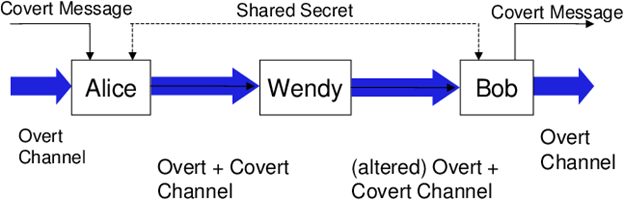
\includegraphics[width=0.9\textwidth]{graphics/chapter-1/Prisoner'problem.png}
    \caption{Tổng quan Bài toán người tù}
    \label{fig:prisonerProblem}
\end{figure*}

Hai cá nhân (Alice và Bob) bị cầm tù. Alice và Bob có thể giao tiếp với nhau, nhưng mọi hoạt động giao tiếp của họ đều bị giám sát liên tục bởi một cai ngục (Wendy). Alice và Bob muốn ấp ủ một kế hoạch trốn thoát, để làm được điều này, họ sẽ sử dụng kỹ thuật ghi mật mã để liên lạc bí mật. Điều quan trọng là thông tin liên lạc của họ không thể bị phát hiện, vì chỉ cần có sự hiện diện của một tin nhắn bí mật sẽ cảnh báo cho Wendy.

\section{Phân loại}
Mức phân loại đầu tiên dựa trên định dạng của video che (cover video). Video che được xem xét thuộc miền thô (Raw domain) hay miền nén (compressed domain). Các video miền thô được phân loại thành miền không gian (spatial domain) và miền biến đổi (transform domain). Phương pháp thay thế Bit ít quan trọng nhất (Least Significant Bits - LSB) và các phương pháp quan trọng khác được bao gồm trong miền không gian. Biến đổi Wavelet rời rạc (DWT) và Biến đổi Cosine rời rạc (DCT) là các phương pháp biến đổi được sử dụng rộng rãi để biến đổi các video che thành miền biến đổi. Sau khi biến đổi video thành miền biến đổi, việc nhúng thông tin bí mật được thực hiện. Trong miền nén, ghi video sử dụng video che nén. Video được nén có ít dung lượng lưu trữ hơn so với video thô và quá trình nhúng diễn ra trong hoặc sau quá trình nén video. Vectơ chuyển động, chế độ dự đoán nội bộ, mô-đun mã hóa entropy, và các kỹ thuật DCT/DST là các phương pháp ghi video được sử dụng rộng rãi trong miền nén. 

Video Steganography có ứng dụng của nó trong các lĩnh vực/lĩnh vực khác nhau, nơi thường sử dụng giao tiếp bí mật. Các lĩnh vực phổ biến mà kỹ thuật giấu tin video được sử dụng là các cơ quan tình báo, quân đội, ngành y tế và đa phương tiện. Các cơ quan tình báo luôn thích giao tiếp bí mật khi họ giao tiếp bên trong cũng như bên ngoài cơ quan. Video Steganography được sử dụng rộng rãi trong trường hợp này khi chúng có thể che giấu sự tồn tại của thông điệp bí mật khỏi kẻ tấn công. Tương tự như các cơ quan tình báo, các tổ chức quân sự cũng đang sử dụng rộng rãi các kỹ thuật steganography để che đậy thông tin liên lạc của họ. Bởi vì việc tiết lộ trái phép dữ liệu bí mật có thể dẫn đến các vấn đề về an ninh quốc gia. Lĩnh vực y tế cũng đã được hưởng lợi từ việc áp dụng kỹ thuật ghi video. Sự tiến bộ hiện nay trong lĩnh vực y tế đã làm cho việc lưu trữ thông tin của bệnh nhân ở dạng kỹ thuật số. Hơn nữa, thông tin này được lưu trữ trên đám mây và có thể được chuyển đến bệnh nhân tương ứng hoặc nhà cung cấp dịch vụ chăm sóc sức khỏe được ủy quyền với sự trợ giúp của kết nối internet. Truyền dữ liệu y tế qua internet là một vấn đề nghiêm trọng vì bất kỳ sự mất mát dữ liệu nào xảy ra do các cuộc tấn công mạng đều có thể ảnh hưởng tiêu cực đến sức khỏe của bệnh nhân. Ngành y tế đang sử dụng các kỹ thuật ghi video để che giấu thông tin cá nhân của họ khỏi các thực thể trái phép khi nó được chuyển qua các kênh liên lạc. Ngoài ra, kỹ thuật ghi video được sử dụng để bảo vệ quyền riêng tư của các cá nhân được ủy quyền được phát hiện trong các chuỗi video do camera giám sát ghi lại. Dữ liệu của các cá nhân được nhúng bên trong các chuỗi video từ camera giám sát. Các đặc điểm chính của bất kỳ phương pháp steganography nào là không thể nhận thấy, bảo mật, mạnh mẽ và khả năng che giấu. Luôn có sự thỏa hiệp giữa tính bảo mật, tính mạnh mẽ và khả năng che giấu của các phương pháp lưu trữ dữ liệu.

\begin{figure*}[!h]
    \centering
    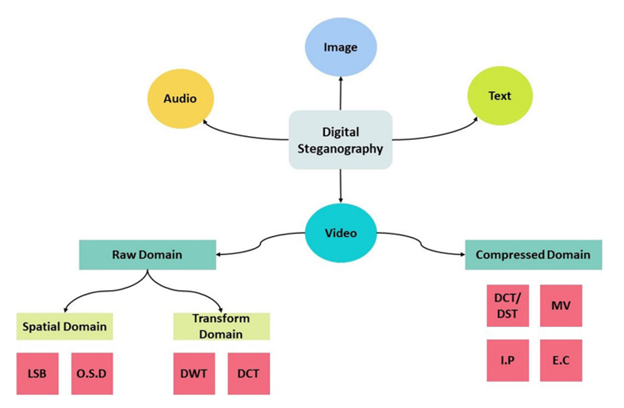
\includegraphics[width=0.9\textwidth]{graphics/chapter-1/Classif_VideoSte.png}
    \caption{Phân loại các dạng Video Steganography}
    \label{fig:classifi}
\end{figure*}

\subsection{Video steganography trong miền thô (Raw domain)}
Các phương pháp ghi video dựa trên miền thô coi video che (cover video) là một chuỗi các khung và thao tác nhúng dữ liệu được áp dụng cho từng khung riêng biệt. Quy trình nhúng dữ liệu chung trong miền thô được hiển thị trong hình \ref{fig:Process_rawdomain} bên dưới. 

\begin{figure*}[!h]
    \centering
    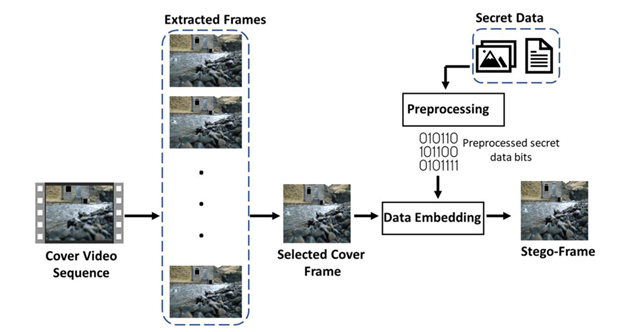
\includegraphics[width=0.9\textwidth]{graphics/chapter-1/Process_rawdomain.png}
    \caption{Quy trình nhúng dữ liệu chung trong miền thô}
    \label{fig:Process_rawdomain}
\end{figure*}

Ban đầu, chuỗi video che (cover video sequence) được chuyển đổi thành nhiều khung hình. Sau đó, dữ liệu bí mật được ẩn bên trong các khung bằng nhiều phương pháp khác nhau. Trong miền thô, dữ liệu bí mật được nhúng trực tiếp vào miền không gian của khung che (cover frame) hoặc khung che được chuyển thành miền tần số (frequency domain) và dữ liệu bí mật được nhúng vào miền tần số. Trước khi nhúng, dữ liệu bí mật phải được tiền xử lý. Nhiều phương pháp đã áp dụng các kỹ thuật mã hóa (encryption techniques), mã sửa lỗi (error-correcting codes),… để xử lý trước dữ liệu bí mật. Quá trình tiền xử lý dữ liệu bí mật được triển khai để đảm bảo tính bảo mật của dữ liệu bí mật ngay cả khi video che bị bất kỳ cuộc tấn công nào hoặc giảm khung hình (frame drops) trong quá trình truyền. 

Phương pháp dựa trên miền thô (raw domain-based method) có thể được phân thành hai loại: ẩn dữ liệu trong miền không gian (Data hiding in spatial domain) và ẩn dữ liệu trong các phương thức miền biến đổi (Data hiding in transform domain).

\begin{itemize}
    \item Ẩn dữ liệu trong miền không gian (Data hiding in spatial domain):
    Các kỹ thuật giấu dữ liệu trong miền không gian sử dụng các giá trị pixel của khung che để giấu dữ liệu bí mật. Nó có nghĩa là các bit dữ liệu bí mật được nhúng trực tiếp vào các giá trị cường độ pixel (pixel intensity values). Các bit ít quan trọng nhất (The least significant bits - LSB) hay  thay thế LSB (LSB substitution) là một phương pháp phổ biến, trong đó các bit dữ liệu bí mật được nhúng vào các bit ít quan trọng nhất của cường độ pixel che phủ (cover pixels intensities), được sử dụng để ẩn dữ liệu trong miền không gian. 
    \begin{itemize}
        \item Các phương pháp LSB:     
Các phương pháp dựa trên các Bit ít quan trọng nhất là thuật toán thường được sử dụng cho kỹ thuật ghi ảnh, âm thanh và video. Các phương pháp LSB rất đơn giản và hiệu quả. Thông thường, các phương thức LSB được mô tả là các phương thức thay thế k-LSB trong đó k là số bit bí mật có thể được ẩn. Dựa trên thuật toán nhúng, giá trị của k được thay đổi. Khả năng ẩn của thuật toán nhúng phụ thuộc vào số bit (k) có thể được thao tác trong video che. Tăng số lượng bit để giấu tin có thể tăng khả năng giấu tin nhưng cũng sẽ làm quá tải cho phương tiện mang tin, dẫn đến việc tiết lộ thông tin bí mật. Bảng \ref{tab:LSB_survey} thể hiện một số nghiên cứu sử dụng phương pháp LSB. Trong bảng \ref{tab:LSB_survey}, \textbf{Imp} thể hiện cho tính không thể nhận thấy; \textbf{Rob} thể hiện cho độ mạnh mẽ; và \textbf{Cap} thể hiện cho khả năng che giấu của thuật toán.

\begin{table}[!h]
\caption{Các nghiên cứu sử dụng phương pháp LSB} 
\label{tab:LSB_survey}
\centering
\resizebox{\textwidth}{!}{%
\begin{tabular}{|c|c|c|c|c|c|}
\hline
\textbf{Year} & \textbf{Method}                               & \textbf{Imp} & \textbf{Rob} & \textbf{Cab} & \textbf{Remarks}         \\ \hline
2019 & 2-LSB \cite{1_younus2019video}                            & + & - & N/A         & Security   is not tested       \\ \hline
2011 & 1-LSB \cite{2_ramalingam2011stego}                            & + & - & N/A         & Security   is not tested       \\ \hline
2011 & 4-LSB  \cite{3_hu2011novel}                           & + & - & 1.5   bpp   & No   obvious visual distortion \\ \hline
2012 & Hash-LSB \cite{4_dasgupta2012hash}                        & + & - & 2.6   bpp   & Low                            \\ \hline
2014 & Hash-LSB \cite{5_kaur2014improved}                         & + & - & 100\%       & Security   is not tested       \\ \hline
2017 & Spiral LSB \cite{6_jha2017video}                      & + & - & 25\%        & Low   hiding capacity          \\ \hline
2020 & Adaptive 4-LSB \cite{7_mstafa2020new}               & + & + & 0.069   bpp & Low   embedding capacity       \\ \hline
2013 & 3–3-2   LSB and Genetic algorithm \cite{8_dasgupta2013optimized} & + & - & 8   bpp     & Security   is low              \\ \hline
2010          & LSB   replacement  and directed graph patterns \cite{9_bhattacharyya2010directed} & -                         & -                   & 2560   KB         & Security   is not tested \\ \hline
\end{tabular}%
}
\end{table}

Một pixel duy nhất trong khung của video bao phủ có từ 8 đến 24 bit dựa trên định dạng của video. Các khung màu xám có 8 bit trong khi một khung màu sắc có 24 bit. Một khung màu sắc bao gồm 3 kênh (RGB) và mỗi kênh bao gồm 8 bit cho mỗi pixel. Tương tự, một khung bí mật RGB của video bao gồm 8 bit cho mỗi pixel cho tất cả 3 kênh. Các bit ít quan trọng nhất của khung bao phủ được thay thế bằng các bit quan trọng nhất của khung bí mật. Trong quá trình trích xuất, các bit LSB của ảnh Stego được lấy ra và các bit 0 được thêm vào để thu được một xấp xỉ thông tin bí mật như ý.
        \item Các phương pháp miền không gian khác:

Hầu hết các kỹ thuật ghi video cho video thô trong miền không gian đều dựa vào sự thay thế LSB để nhúng dữ liệu bí mật. Bên cạnh đó, một số công trình được đề xuất trong thập kỷ qua đã sử dụng các phương pháp không phải LSB để ẩn dữ liệu bí mật trong miền không gian của video thô.


Hầu hết LSB và các phương pháp miền không gian khác đều đạt được khả năng che giấu dữ liệu cũng như khả năng che giấu dữ liệu chấp nhận được. Tuy nhiên, tính mạnh mẽ của các phương pháp được đề xuất là một mối quan tâm và nhiều phương pháp chưa tiến hành bất kỳ phân tích định lượng nào để đánh giá tính mạnh mẽ của chúng. Hầu hết các phương pháp dựa trên miền không gian dễ bị tấn công phân tích dữ liệu và không đủ mạnh để chống lại các cuộc tấn công nén (compression attack) cũng như tấn công nhiễu (noise attack).

    \end{itemize}
    \item Ẩn dữ liệu trong miền biến đổi (Data hiding in transform domain):
    Không giống như phương pháp dựa trên miền không gian nhúng trực tiếp dữ liệu bí mật vào cường độ pixel thô của pixel che (cover pixel), phương pháp dựa trên miền biến đổi biến đổi các khối của khung che trong miền không gian sang miền biến đổi. Sau đó, dữ liệu bí mật được nhúng vào các bit có ý nghĩa nhỏ nhất của hệ số biến đổi. Quy trình chung của việc ẩn dữ liệu trong miền biến đổi được thể hiện trong Hình \ref{fig:Process_transform}. Biến đổi wavelet rời rạc (Discrete Wavelet Transform - DWT) và biến đổi cosine rời rạc ( Discrete Cosine Transform - DCT) là hai hàm biến đổi được sử dụng chủ yếu trong kỹ thuật ghi video.

\begin{figure*}[!h]
    \centering
    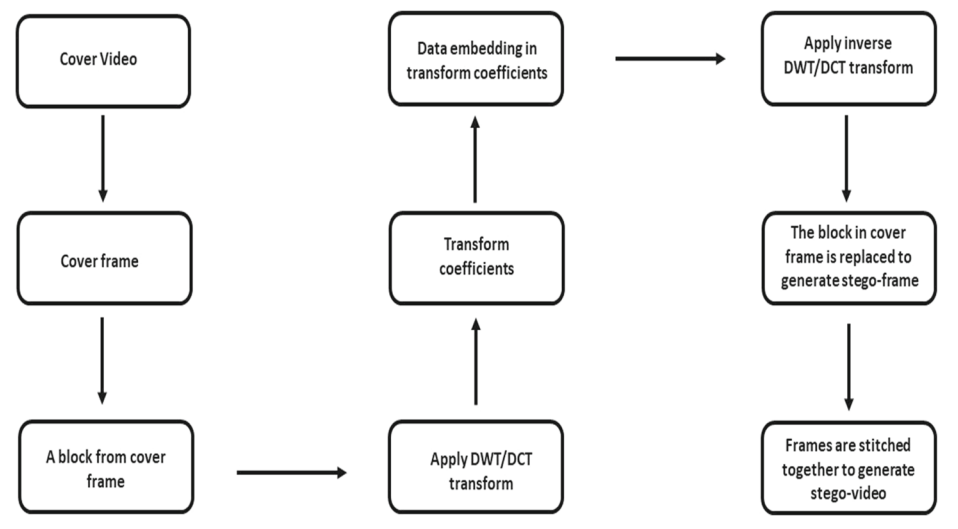
\includegraphics[width=0.9\textwidth]{graphics/chapter-1/transform_overview.PNG}
    \caption{Quy trình nhúng dữ liệu chung trong miền biến đổi}
    \label{fig:Process_transform}
\end{figure*}

    \begin{itemize}
        \item Biến đổi wavelet rời rạc (Discrete Wavelet Transform - DWT):
Một kỹ thuật miền biến đổi khác được sử dụng cho kỹ thuật ghi video là DWT, trong đó quá trình nhúng được thực hiện bằng cách phân tách các khung thành các cấp độ khác nhau. Mỗi cấp độ được chia thành bốn phần tần số, tức là LL, LH, HL và HH trong đó chỉ có một (LL) là thành phần tần số cấp thấp và ba thành phần còn lại là thành phần tần số cấp cao. Nói chung, băng con/thành phần LL được phân tách lặp lại thành các cấp độ cao hơn (Faragallah 2013); tuy nhiên, các băng con khác cũng có thể được phân tách thành các mức khác nhau. Kết quả triển khai phân tách 2D DWT một cấp và hai cấp (băng con LL) trên khung của định dạng video CIF (Định dạng trung gian chung) từ tập dữ liệu dấu vết phổ biến (Reisslein 2012) với độ phân giải 352×288 được hiển thị trong Hình .12.
DWT là một kỹ thuật toán học thường được sử dụng trong xử lý tín hiệu và nén ảnh. Trong phép biến đổi DWT hai chiều, một ảnh gốc I sẽ được phân tích thành bốn băng tần có kích thước bằng $1/2$ ảnh gốc: LL (low frequency component in horizontal and vertical direction), LH (low frequency component in horizontal direction and high frequency in vertical direction), HL (high frequency component in horizontal direction and low frequency in vertical direction), HH (high frequency component in horizontal direction and high frequency in vertical direction).

        \item Biến đổi cosine rời rạc ( Discrete Cosine Transform - DCT):

DCT cũng là một chức năng biến đổi giống như DWT, chia hình ảnh thành các băng con quang phổ. Sự khác biệt chính giữa DCT và DWT là loại trước đó tạo ra nhiều dải tần hơn và cung cấp độ phân giải tần số cao hơn. Tuy nhiên, DWT tạo ra một vài dải tần số và cung cấp độ phân giải không gian cao. Một số lượng đáng kể các tác phẩm trong tài liệu đã sử dụng miền DWT để nhúng dữ liệu bí mật vào các video thô. Không giống như DWT, miền DCT không được sử dụng thường xuyên trong tài liệu để ẩn dữ liệu bí mật bên trong video thô . Mặt khác, các phương pháp ghi video được đề xuất trong miền nén đã sử dụng rộng rãi miền DCT để ẩn dữ liệu bí mật.

    \end{itemize}
\end{itemize}

Bảng \ref{tab:DCT_DWT_survey} thể hiện một số nghiên cứu sử dụng phương pháp DCT và DWT. Trong bảng \ref{tab:DCT_DWT_survey}, \textbf{Imp} thể hiện cho tính không thể nhận thấy; \textbf{Rob} thể hiện cho độ mạnh mẽ; và \textbf{Cap} thể hiện cho khả năng che giấu của thuật toán.

\begin{table}[!h]
\centering
\caption{Các nghiên cứu sử dụng phương pháp DCT và DWT} 
\label{tab:DCT_DWT_survey}
\resizebox{\textwidth}{!}{%
\begin{tabular}{|c|c|c|c|c|c|}
\hline
\textbf{Year} &
  \textbf{Method} &
  \textbf{Imp} &
  \textbf{Rob} &
  \textbf{Cab} &
  \textbf{Remarks} \\ \hline
2014 & DWT,   DCT \& LSB \cite{11_ahmed2014information} & + & + & 1.8   KB    & Security   is not tested                       \\ \hline
2016 & DWT   \& LSB \cite{12_kolakalur2016wavelet}      & + & - & N/A         & Evaluated   in multiple video formats          \\ \hline
2017 &
  DWT   \& LSB \cite{13_sushmitha2017approach} &
  + &
  - &
  N/A &
  Able   to hide multiple videos inside single video with minimal visual distortion \\ \hline
2010 & DWT \cite{14_lu2010effective}              & + & + & N/A         & Biometric   image sets are hidden inside video \\ \hline
1997 & DCT \cite{15_swanson1997data}               & + & + & 74.97   KB  & Security   is not tested                       \\ \hline
2019 & 1D-DCT \cite{16_rabie2019pixogram}            & + & + & 16.64   bpp & Security   is not tested                       \\ \hline
2017 &
  Adaptive   method (DWT \& DCT) \cite{17_mstafa2017robust} &
  + &
  + &
  3.40\% &
  Secure   against state of art steganalysis attacks. \\ \hline
\end{tabular}%
}
\end{table}

\subsection{Video steganography trong miền nén (Compressed domain)}
Phần lớn các phương pháp ghi video để ẩn dữ liệu trong miền thô đều đơn giản và dễ thực hiện. Tuy nhiên, chúng dễ bị tấn công hơn, đặc biệt là các cuộc tấn công nén. Hơn nữa, hiện tại, các video ở dạng nén được ưa chuộng hơn để lưu trữ cũng như truyền qua internet. Video nén cần ít dung lượng lưu trữ hơn so với video không nén. Và việc truyền video ở dạng nén qua internet sẽ nhanh hơn và cần ít băng thông hơn. Trong bối cảnh này, các kỹ thuật ẩn dữ liệu trong miền video nén đã trở nên phổ biến trong hai thập kỷ qua. Mặt khác, quá trình nén sẽ loại bỏ dữ liệu video dư thừa và giảm không gian để ẩn nhiều dữ liệu hơn.

Trong miền nén, việc ẩn dữ liệu được thực hiện theo hai cách; ẩn dữ liệu cùng với quy trình mã hóa video và ẩn dữ liệu trong luồng bit được mã hóa. Các kỹ thuật che giấu dữ liệu cùng với quy trình mã hóa video sử dụng các yếu tố cú pháp khác nhau liên quan đến tác vụ mã hóa video để nhúng dữ liệu bí mật. Đối với cách còn lại - các phương pháp ẩn dữ liệu trong luồng bit - sẽ được mã hóa khai thác các mô-đun mã hóa entropy để mang dữ liệu bí mật.

\section{Đặc trưng của Video steganography}
Đánh giá các phương pháp steganography video là rất quan trọng để xác định hiệu suất và hiệu quả của phương pháp. Các tính năng chính được mong đợi từ các phương pháp lưu trữ dữ liệu tốt thường là tính không thể nhận thấy (Imperceptibility), Khả năng che giấu (Hiding capacity), bảo mật (security), Độ mạnh mẽ (Robustness) và khả năng chống lại các cuộc tấn công phân tích dữ liệu khác.
\subsection{Tính không thể nhận thấy (Imperceptibility)}
Khả năng che giấu đo lường khả năng của phương pháp steganography video để nhúng một lượng dữ liệu ẩn vào video mà không gây ra thay đổi đáng kể đối với các đặc điểm chính của video. Phương pháp với khả năng che giấu tốt sẽ cho phép nhúng một lượng lớn dữ liệu mà vẫn duy trì tính tự nhiên và không gây nghi ngờ cho người xem. Tuy nhiên, việc tăng khả năng che giấu có thể dẫn đến việc giảm tính không thể nhận thấy và độ mạnh mẽ của phương pháp.
\subsection{Khả năng che giấu (Hiding capacity)}
Tính không thể nhận thấy là khả năng của phương pháp steganography video để duy trì hình ảnh và âm thanh của video một cách tự nhiên, mà không có sự thay đổi đáng kể. Người xem không nên có khả năng nhận ra sự hiện diện của dữ liệu ẩn trong video một cách dễ dàng. Tính không thể nhận thấy quan trọng để đảm bảo rằng việc ẩn dữ liệu không làm giảm chất lượng trải nghiệm của người xem.
\subsection{Độ mạnh mẽ (Robustness)}
Độ mạnh mẽ của phương pháp steganography video đo lường khả năng của nó chống lại các biến đổi, nhiễu và tấn công mục tiêu mà có thể làm lộ dữ liệu ẩn. Phương pháp mạnh mẽ sẽ duy trì khả năng che giấu và tính không thể nhận thấy ngay cả khi video trải qua các biến đổi như nén ảnh, nén âm thanh, hoặc các cuộc tấn công như tấn công phân tích dữ liệu. Điều này đảm bảo rằng dữ liệu ẩn vẫn an toàn và không bị phát hiện trong các tình huống thực tế.
